\newpage

%%%%%%%%%%%%%%%%%  A1

\begin{justify}
    {\bf  Α.1}\\
    Να δημιουργήσετε παλμούς $SRRC$ $\phi(t)$.\\\\
    {\bf (α)} (5) Να σχεδιαστούν σε κοινό
     \textlatin{plot} οι παλμοί, για $T=10^{-2}, over=10, A=4$ και συντελεστή
    \textlatin{roll-off} $a=0,0.5,1$ στον κατάλληλο άξονα του χρόνου.
\end{justify}

\begin{justify}
    {\bf  (β)} (5) Τι παρατηρείτε σχετικά με τον ρθυμό μείωσης
    του πλάτους των παλμών, όσο αυξάνεται η απόλυτη τιμή του
    χρόνου, $|t|$, σε σχέση με τις τιμές του $a$\textlatin{;}
    Ποιός παλμός
    φθίνει πιο γρήγορα\textlatin{;}\\\\
    \textbf{Λύση:}\\
\end{justify}

%%%%%%PLOT
\begin{center}
    \centering
    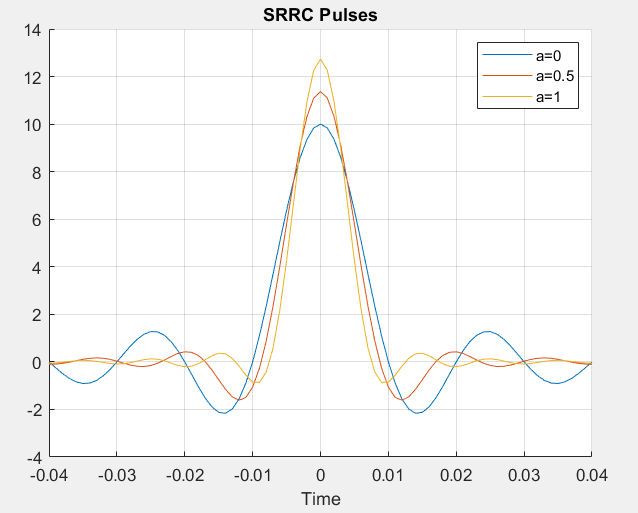
\includegraphics[width=0.8\textwidth]{ALPHA/Images/A1.png} % Adjust width as neededfilename of your images
\end{center}

\begin{justify}
    Ακολουθεί ο κώδικας \textlatin{Matlab}:
\end{justify}

\vspace{-0.5cm}


%%%%%%%%MATLAB code
\textlatin{
    \lstinputlisting[language=Matlab,]{ALPHA/Matlab/a1.m}
}


\begin{justify}
    Παρατηρούμε ότι όσο μειώνεται το $a$ τόσο μειώνεται και ο ρυθμός μείωσης του πλάτους.Άρα
    ο ρυθμός μείωσης του πλάτους είναι αντιστρόφως ανάλογος του συντελεστή \textlatin{roll-off} $a$.
\end{justify}


%%%%%%%%%%%%%%%%%  A2
\vspace{0.5cm}

\begin{justify}
    {\bf  Α.2}\\
    Μέσω των συναρτήσεων \textlatin{fft} και \textlatin{fftshit}
    να υπολογίσετε τους μετασχηματισμους \textlatin{Fourier} $\Phi(F)$ 
    των παλμών που σχεδιάστηκαν στο ερώτημα Α.1,
    σε $N\textsubscript{f}$ ισαπέχοντα σημεία στον άξονα συχνοτήτων 
    $[-\frac{F\textsubscript{s}}{2},\frac{F\textsubscript{s}}{2})$ (ενδεικτικά, $N\textsubscript{f}=1024,2048$).\\\\
    {\bf (α)} (5) Σε κοινό \textlatin{plot}:\\
    {\bf (β)} (5) Σε κοινό \textlatin{semilogy}:
\end{justify}

\newpage

\begin{justify}
    \textbf{Λύση:}\\
    \textbf{(α)}
\end{justify}

%%PLOTS
\begin{minipage}[t]{0.5\textwidth}
    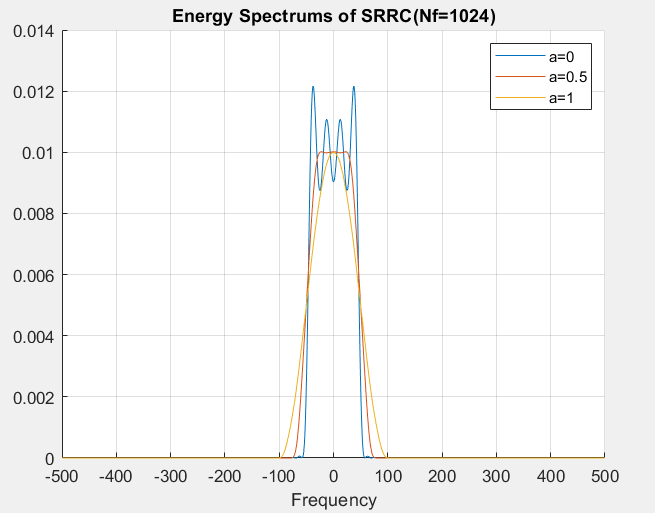
\includegraphics[width=\textwidth]{ALPHA/Images/A1.1024.png}
\end{minipage}
\hfill
\begin{minipage}[t]{0.49\textwidth}
    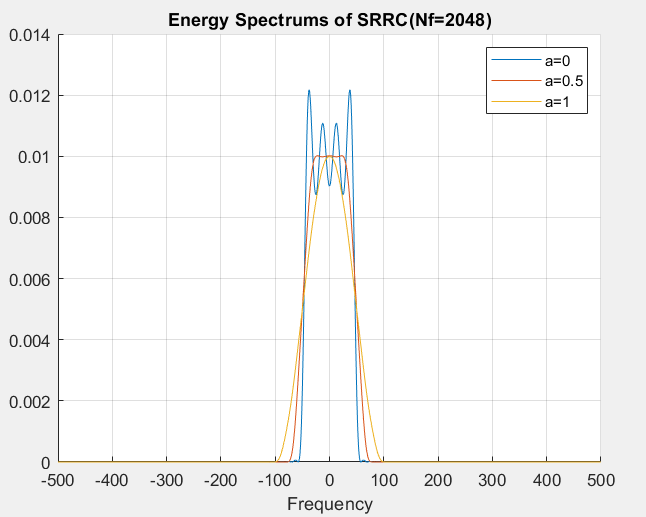
\includegraphics[width=\textwidth]{ALPHA/Images/A1.2048.png}
\end{minipage}

\begin{justify}
    \textbf{(β)}
\end{justify}

%%PLOTS
\begin{minipage}[t]{0.49\textwidth}
    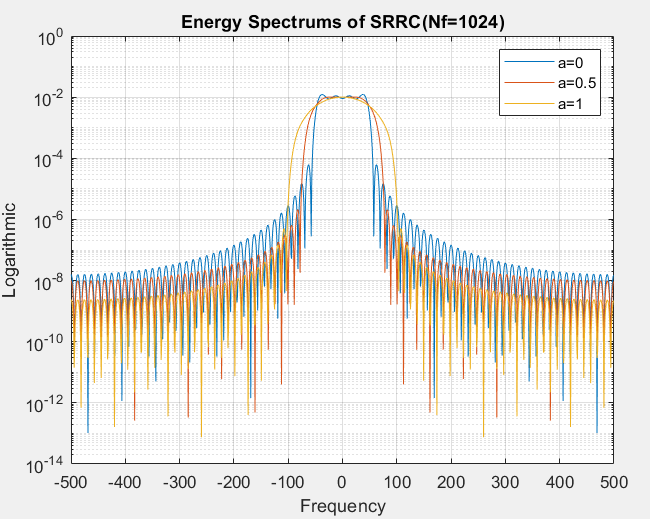
\includegraphics[width=\textwidth]{ALPHA/Images/A1.sem.1024.png}
\end{minipage}
\hfill
\begin{minipage}[t]{0.5\textwidth}
    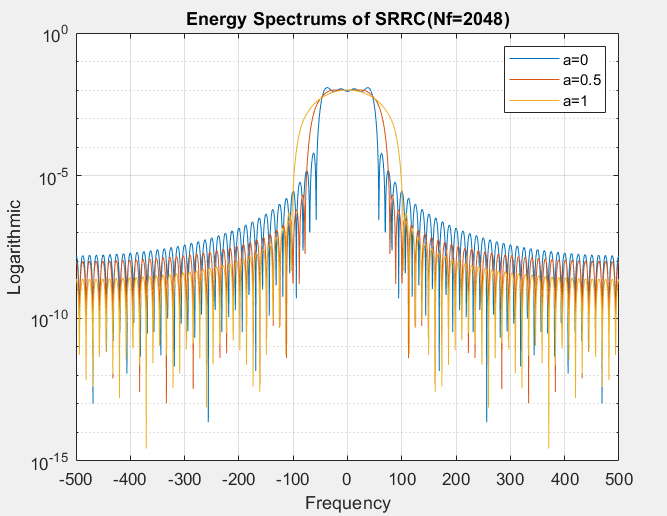
\includegraphics[width=\textwidth]{ALPHA/Images/A1.sem.2048.png}
\end{minipage}

\begin{justify}
    Ακολουθεί ο κώδικας \textlatin{Matlab}:
\end{justify}

\vspace{-0.5cm}

%%%%%%%%MATLAB code
\textlatin{
    \lstinputlisting[language=Matlab,]{ALPHA/Matlab/a2.m}
}


%%%%%%%%%%%%%%%%%  A3
\vspace{0.5cm}

\begin{justify}
    {\bf  Α.3}\\
    Το θεωρητικό εύρος φάσματος των παλμών άπειρης διάρκειας είναι
    $BW =  \frac{1+a}{2T}$.\\\\
    {\bf (a)} (5) Να υπολογίσετε την τιμή του θεωριτικού εύρους φάσματος
    για κάθε ένα από τους τρείς παλμούς:\\\\
    \textbf{Λύση:}\\
\end{justify}


%%%%%%Table 2x4
\begin{table}[htbp]
	\centering
    \begin{tabular}{|c|c|c|c|}
        \hline
        α & 0 & 0.5 & 1\\
        \hline 
        \textlatin{BW} & 50  & 75 & 100   \\
        \hline 
    \end{tabular}
\end{table}

\newpage

\begin{justify}
    {\bf (β)} (5) Στο κοινό \textlatin{semilogy}
    του ερωτήματος Α.2, να σχεδιάσετε μία οριζόντια γραμμή με $c$
    με τιμή $c=\frac{T}{10^{3}}$ και να θεωρήσετε ότι οι τιμές 
    οι οποίες ευρίσκονται κάτω από αυτή τη γραμμή είναι πρακτικά μηδέν.
    Σε αυτή την περίπτωση, ποιο είναι προσεγγιστικά το εύρος
    φάσματος των τριών παραπάνω παλμώn\textlatin{;} Ποιός
    παλμός είναι πιο αποδοτικός ως προς το εύρος φάσματος\textlatin{;}\\\\
    \textbf{Λύση:}\\
    Tο πρακτικό εύρος φάσματος είναι προσεγγιστικά:
\end{justify}

%%%%%%Table 2x4
\begin{table}[htbp]
	\centering
    \begin{tabular}{|c|c|c|c|}
        \hline
        α & 0 & 0.5 & 1\\
        \hline 
        \textlatin{BW} & 77.6  & 75.6 & 98.6\\
        \hline 
    \end{tabular}
\end{table}

\begin{justify}
    Έτσι παρατηρούμε ότι ο παλμός με $a=0.5$ είναι ο πιο αποδοτικός διότι
    έχει πρακτικά το μικρότερο εύρος φάσματος.\\\\
    {\bf (γ)} (5) Πώς μεταβάλλεται το εύρος φάσματος των παλμών αν 
    $c=\frac{T}{10^{5}}$\textlatin{;} Σε αυτήν την περίπτωση
    ποιός παλμός είναι πιο αποδοτικός\textlatin{;}\\\\
    \textbf{Λύση:}\\
\end{justify}

%%%%%%Table 2x4
\begin{table}[htbp]
	\centering
    \begin{tabular}{|c|c|c|c|}
        \hline
        α & 0 & 0.5 & 1\\
        \hline 
        \textlatin{BW} & 213.8  & 132.3 & 121.1\\
        \hline 
    \end{tabular}
\end{table}

\begin{justify}
    Σε αυτήν την περίπτωση ο παλμός με $a=1$ είναι πιο αποδοτικός.
\end{justify}

\newpage

\begin{justify}
    Ακολουθεί κοινό \textlatin{plot} και ο κώδικας \textlatin{Matlab}:
\end{justify}

%%%%%%PLOT
\begin{center}
    \centering
    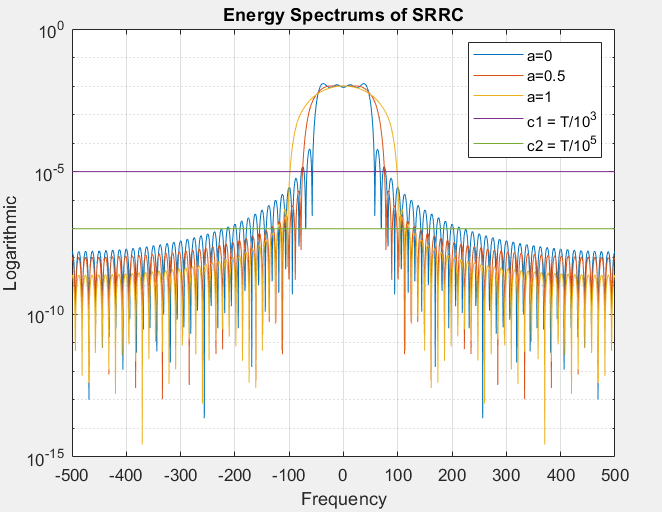
\includegraphics[width=0.8\textwidth]{ALPHA/Images/A3.png} % Adjust width as neededfilename of your images
\end{center}

%%%%%%%%MATLAB code
\textlatin{
    \lstinputlisting[language=Matlab,]{ALPHA/Matlab/a3.m}
}
